\documentclass[border={5pt 0pt}]{standalone}

\usepackage{xcolor}
\definecolor{fgcolor}{HTML}{f0f6fc}
\definecolor{bgcolor}{HTML}{0d1117}
\definecolor{myblue}{HTML}{1d597f}
\definecolor{myorange}{HTML}{b27b43}
\definecolor{mygreen}{HTML}{699963}
\colorlet{mygray}{gray!50!black}

\usepackage{tikz}
\usepackage{tikz-timing}
\usetikzlibrary{fit, positioning, shapes.geometric, shapes.symbols, backgrounds}

\newlength{\vhdlregh}\setlength{\vhdlregh}{2em}
\newlength{\vhdlregw}\setlength{\vhdlregw}{1em}

\tikzset{
    text=fgcolor,
    arrow/.style={ ->, draw=fgcolor, very thick },
    % Register
    regbox/.style={ rectangle, very thick, draw=fgcolor, fill=mygray, minimum width=\vhdlregw, minimum height=\vhdlregh },
    regwedge/.style={ isosceles triangle, isosceles triangle apex angle=80, draw=fgcolor, very thick, anchor=right corner, scale=0.33 },
    register/.pic={
        \node[regbox] () {#1};
        \node[above right=0.1em and 0.05em of .south west, regwedge] (-wedge) {};
    },
    % Adder, multiplier, etc.
    adder/.style={ circle, draw=fgcolor, very thick },
    % Cloud (for combinational logic)
    mycloud/.style={ cloud, draw=fgcolor, very thick, inner sep=2pt, minimum width=0.8cm, minimum height=0.8cm },
}


\usepackage{pifont}
\newcommand{\mycheckmark}{\ding{52}}
\newcommand{\mycrossmark}{\ding{56}}

\usepackage{bm}

\begin{document}

\pagecolor{bgcolor}

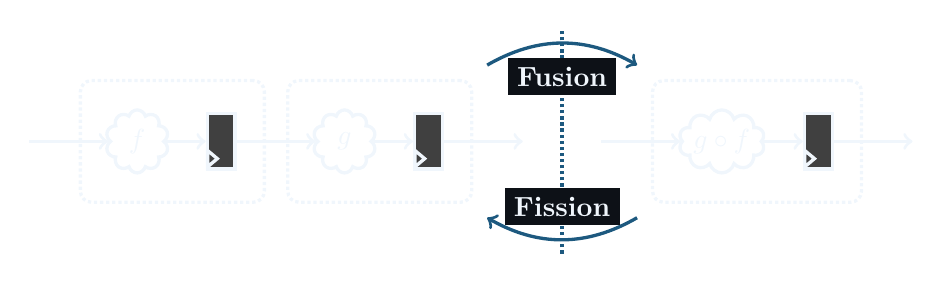
\begin{tikzpicture}
    % Before fusion
    \coordinate (start);
    \node[mycloud, right=of start] (f) {$f$};
    \pic[right=0.5 of f] (reg-f) {register};
    \node[mycloud, right=of reg-f] (g) {$g$};
    \pic[right=0.5 of g] (reg-g) {register};
    \coordinate[right=of reg-g] (end);
    \node[draw=fgcolor, densely dotted, very thick, fit=(f) (reg-f), rounded corners, inner sep=1em] (entity-f) {};
    \node[draw=fgcolor, densely dotted, very thick, fit=(g) (reg-g), rounded corners, inner sep=1em] (entity-g) {};

    \draw[arrow] (start) to (f);
    \draw[arrow] (f) to (reg-f);
    \draw[arrow] (reg-f) to (g);
    \draw[arrow] (g) to (reg-g);
    \draw[arrow] (reg-g) to (end);

    % After fusion
    \coordinate[right=of end] (start);
    \node[mycloud, aspect=2, inner sep=0, right=of start] (fg) {$g \circ f$};
    \pic[right=0.5 of fg] (reg-fg) {register};
    \coordinate[right=of reg-fg] (end);
    \node[draw=fgcolor, densely dotted, very thick, fit=(fg) (reg-fg), rounded corners, inner sep=1em] (entity-fg) {};

    \draw[arrow] (start) to (fg);
    \draw[arrow] (fg) to (reg-fg);
    \draw[arrow] (reg-fg) to (end);

    % Separator + arrows back and forth
    \draw[arrow, myblue] ([xshift=5pt, yshift=5pt] entity-g.north east) to[bend left=30] coordinate[midway] (vrule-top) ([xshift=-5pt, yshift=5pt] entity-fg.north west);
    \draw[arrow, myblue] ([xshift=-5pt, yshift=-5pt] entity-fg.south west) to[bend left=30] coordinate[midway] (vrule-bot) ([xshift=5pt, yshift=-5pt] entity-g.south east);
    \draw[arrow, -, myblue, densely dotted] ([xshift=0pt, yshift=-5pt] vrule-bot) to ([xshift=0pt, yshift=5pt] vrule-top);
    \node[below=5pt of vrule-top, fill=bgcolor, text=fgcolor] {\textbf{Fusion}};
    \node[above=5pt of vrule-bot, fill=bgcolor, text=fgcolor] {\textbf{Fission}};
\end{tikzpicture}

\end{document}
